\section{Question 1 (40 points)} 
Suppose we have a single-layer model with only one neuron as shown in the figure below, with a sigmoid activation function.

\begin{figure}[H]
    \centering
    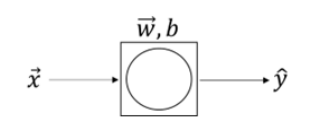
\includegraphics[width=0.6\textwidth]{Q1_rep.png}
\end{figure}

For a binary classification problem, we consider the following cost function for learning:

\[
E_{w, b} = -\sum_n \left[ y_n \ln \hat{y}(x_n) + (1 - y_n) \ln (1 - \hat{y}(x_n)) \right]
\]

Show that the cost function has a minimum. Then, write an equation to reach the minimum point.
\begin{qsolve}
    \begin{qsolve}[]
        The cost function \( E_{w,b} \) represents the binary cross-entropy loss, which is a convex function with respect to the parameters \( w \) and \( b \). to prove the convexity of the function, we need to show that the Hessian matrix of the function is positive semi-definite. we have:
        \[
        E_{w,b} = -\sum_n \left[ y_n \ln \hat{y}(x_n) + (1 - y_n) \ln (1 - \hat{y}(x_n)) \right]
        \]

        where \( y_n \in \{0, 1\} \) is the true label, and \( \hat{y}(x_n) = \sigma(w^T x_n + b) \) is the prediction, with \( \sigma(z) = \frac{1}{1 + e^{-z}} \) being the sigmoid function.
        \[
        \hat{y} = \sigma(w^T x + b) = \frac{1}{1 + e^{-(w^T x + b)}}
        \]
        \[
        E_n = - \left[ y_n \ln \hat{y} + (1 - y_n) \ln (1 - \hat{y}) \right]
        \]
        \splitqsolve[\splitqsolve]
        now we can calculate first and second derivatives of the cost function with respect to the parameters \( w \) and \( b \) to find the minimum point.
        \[
        \frac{\partial \hat{y}}{\partial w} = \hat{y}(1 - \hat{y}) x
        \]
        \[
        \frac{\partial E_n}{\partial w} = -\left( \frac{y_n}{\hat{y}} - \frac{1 - y_n}{1 - \hat{y}} \right) \frac{\partial \hat{y}}{\partial w}
        \]
        Substituting \( \frac{\partial \hat{y}}{\partial w} = \hat{y}(1 - \hat{y}) x \):
        \[
        \frac{\partial E_n}{\partial w} = ( \hat{y} - y_n ) x
        \]
        The second derivative (Hessian) of \( E_n \) with respect to \( w \) is:
        \[
        \frac{\partial^2 E_n}{\partial w \partial w^T} = \frac{\partial}{\partial w} \left( ( \hat{y} - y_n ) x \right)
        \]
        Since \( \hat{y} = \sigma(w^T x + b) \), taking the derivative of \( \hat{y} - y_n \) with respect to \( w \) gives:
        \[
        \frac{\partial^2 E_n}{\partial w \partial w^T} = \hat{y}(1 - \hat{y}) x x^T
        \]
        The Hessian matrix of the cost function is:
        \[
        H = \sum_n \hat{y}(1 - \hat{y}) x_n x_n^T
        \]
        since the term \( \hat{y}(1 - \hat{y}) \) is always positive and \( x_n x_n^T \) is a positive semi-definite matrix, the Hessian matrix is positive semi-definite and the cost function is convex in respect to the parameters \( w \). now we do the same for the parameter \( b \):
        \[
        \frac{\partial \hat{y}}{\partial b} = \hat{y}(1 - \hat{y})
        \] 
        \[
        \Rightarrow \frac{\partial E_{w, b}}{\partial b} = -\sum_n \left[ \frac{y_n}{\hat{y}} - \frac{1 - y_n}{1 - \hat{y}} \right] \frac{\partial \hat{y}}{\partial b}
        \]
        Substituting \( \frac{\partial \hat{y}}{\partial b} = \hat{y}(1 - \hat{y}) \):
        \[
        \frac{\partial E_{w, b}}{\partial b} = \sum_n (\hat{y} - y_n)
        \]
        Now, let’s compute the second derivative of \( E_{w, b} \) with respect to \( b \).
        \[
        \frac{\partial^2 E_{w, b}}{\partial b^2} = \frac{\partial}{\partial b} \left( \sum_n (\hat{y} - y_n) \right)
        \]
        Since \( \hat{y} = \sigma(w^T x_n + b) \), we have:
        \[
        \frac{\partial^2 E_{w, b}}{\partial b^2} = \sum_n \frac{\partial \hat{y}}{\partial b}
        \]
        \splitqsolve[\splitqsolve]
        Using \( \frac{\partial \hat{y}}{\partial b} = \hat{y}(1 - \hat{y}) \):
        \[
        \frac{\partial^2 E_{w, b}}{\partial b^2} = \sum_n \hat{y}(1 - \hat{y})
        \]
        The Hessian matrix of the cost function is:
        \[
        H = \sum_n \hat{y}(1 - \hat{y})
        \]
        Since the term \( \hat{y}(1 - \hat{y}) \) is always positive, the Hessian matrix is positive semi-definite and the cost function is convex in respect to the parameter \( b \). Therefore, the cost function has a minimum point. To reach the minimum point, we can use the gradient descent algorithm to update the parameters \( w \) and \( b \) iteratively:
        \[
        w \leftarrow w - \eta \sum_n \left( \hat{y}(x_n) - y_n \right) x_n
        \]
        \[
        b \leftarrow b - \eta \sum_n \left( \hat{y}(x_n) - y_n \right)
        \]
    \end{qsolve}
\end{qsolve}